\section{Results}
\paragraph{Experimental Setup and Evaluation.}
We evaluate our method on multiple multi-batch single-cell and spatial transcriptomics datasets. 
For single-cell data, we use (i) a Pancreas dataset (10k cells, 9 batches, 16 cell types), 
(ii) an Immune dataset (30k cells, 5 datasets, 9 cell types), and (iii) a Lung dataset [add details]. 
For spatial data, we use a Non-Small Cell Lung Cancer (NSCLC) dataset, training on a single slide comprising $x$ cell types and $y$ distinct niche labels. For computational efficiency, we subsample up to 30k cells using stratified sampling over both cell types and niches.

We construct cell--cell affinity graphs to define the structure to be preserved.
For transcriptomic experiments, affinities are computed using an adaptive Gaussian kernel on PCA embeddings, following prior work~\cite{seacell}. 
For spatial experiments, we compute affinities using the same adaptive Gaussian kernel, but applied to spatially aggregated features obtained by averaging the features of neighboring cells within a fixed spatial radius, thereby incorporating microenvironmental structure into the affinity.

We compare against (i) SEACells, a state-of-the-art metacell method based on archetypal analysis, 
(ii) a reconstruction-only baseline (CVAE) to isolate the effect of affinity guidance, and 
(iii) parametric UMAP, which preserves the geometry of the data by aligning pairwise relationships in the embedding space. 
For spatial experiments, we additionally evaluate SEACells using the same spatial affinity to ensure a fair comparison.

\paragraph{Evaluation Protocol.}
We evaluate SCProto through a sequence of analyses aligned with our design goals.
First, we assess whether the model preserves the community structure of the input affinity graph using modularity.
Second, we evaluate whether SCProto enables cross-batch aggregation by measuring the batch entropy of each metacell.
Third, we examine whether this cross-batch alignment preserves biological signal using cell-type purity. We then focus on underrepresented populations and evaluate performance on rare cell types, measuring both their coverage—i.e., whether each rare cell type is represented by at least one metacell—and the purity of the corresponding metacells.

Finally, for spatial data, we evaluate whether training on spatially derived affinities enables SCProto to capture microenvironmental signals that are not recoverable from transcriptomic similarity alone. We assess this using cell-type and niche purity of the learned metacells, and visualize the resulting spatial organization.

\subsection{SCProto preserves graph structure and forms cross-batch metacells}
We evaluate whether SCProto simultaneously (i) preserves the community structure of the input affinity graph, (ii) aligns cells across batches, and (iii) maintains biological identity. To this end, we measure modularity of the learned clusters with respect to the input graph, batch entropy of each metacell, and cell-type purity.

As shown in Table~\ref{tab:graph_batch}, SCProto achieves modularity comparable to SEACells, indicating that it preserves the community structure of the input affinity graph. At the same time, it exhibits substantially higher batch entropy, demonstrating effective mixing of cells across batches. Importantly, this is achieved without compromising biological identity, as SCProto maintains cell-type purity comparable to competing methods.

In contrast, SEACells attains similar modularity and purity but exhibits very low batch entropy, indicating that it forms batch-specific metacells without meaningful cross-batch aggregation. Conversely, CVAE and parametric UMAP achieve high batch entropy and purity but show significantly lower modularity, suggesting that they fail to preserve the community structure encoded in the affinity graph.

These differences are further illustrated in Fig.~\ref{fig:pancreas_umap}, where UMAP visualizations of pancreas metacells show that SCProto forms clusters that are well aligned across batches while remaining consistent with cell-type structure, whereas SEACells produces clusters that are largely separated by batch.

Together, these results demonstrate that SCProto uniquely balances structure preservation and cross-batch alignment, enabling the formation of biologically coherent metacells that respect the input graph while aggregating information across batches.

\begin{figure*}[t]
\centering
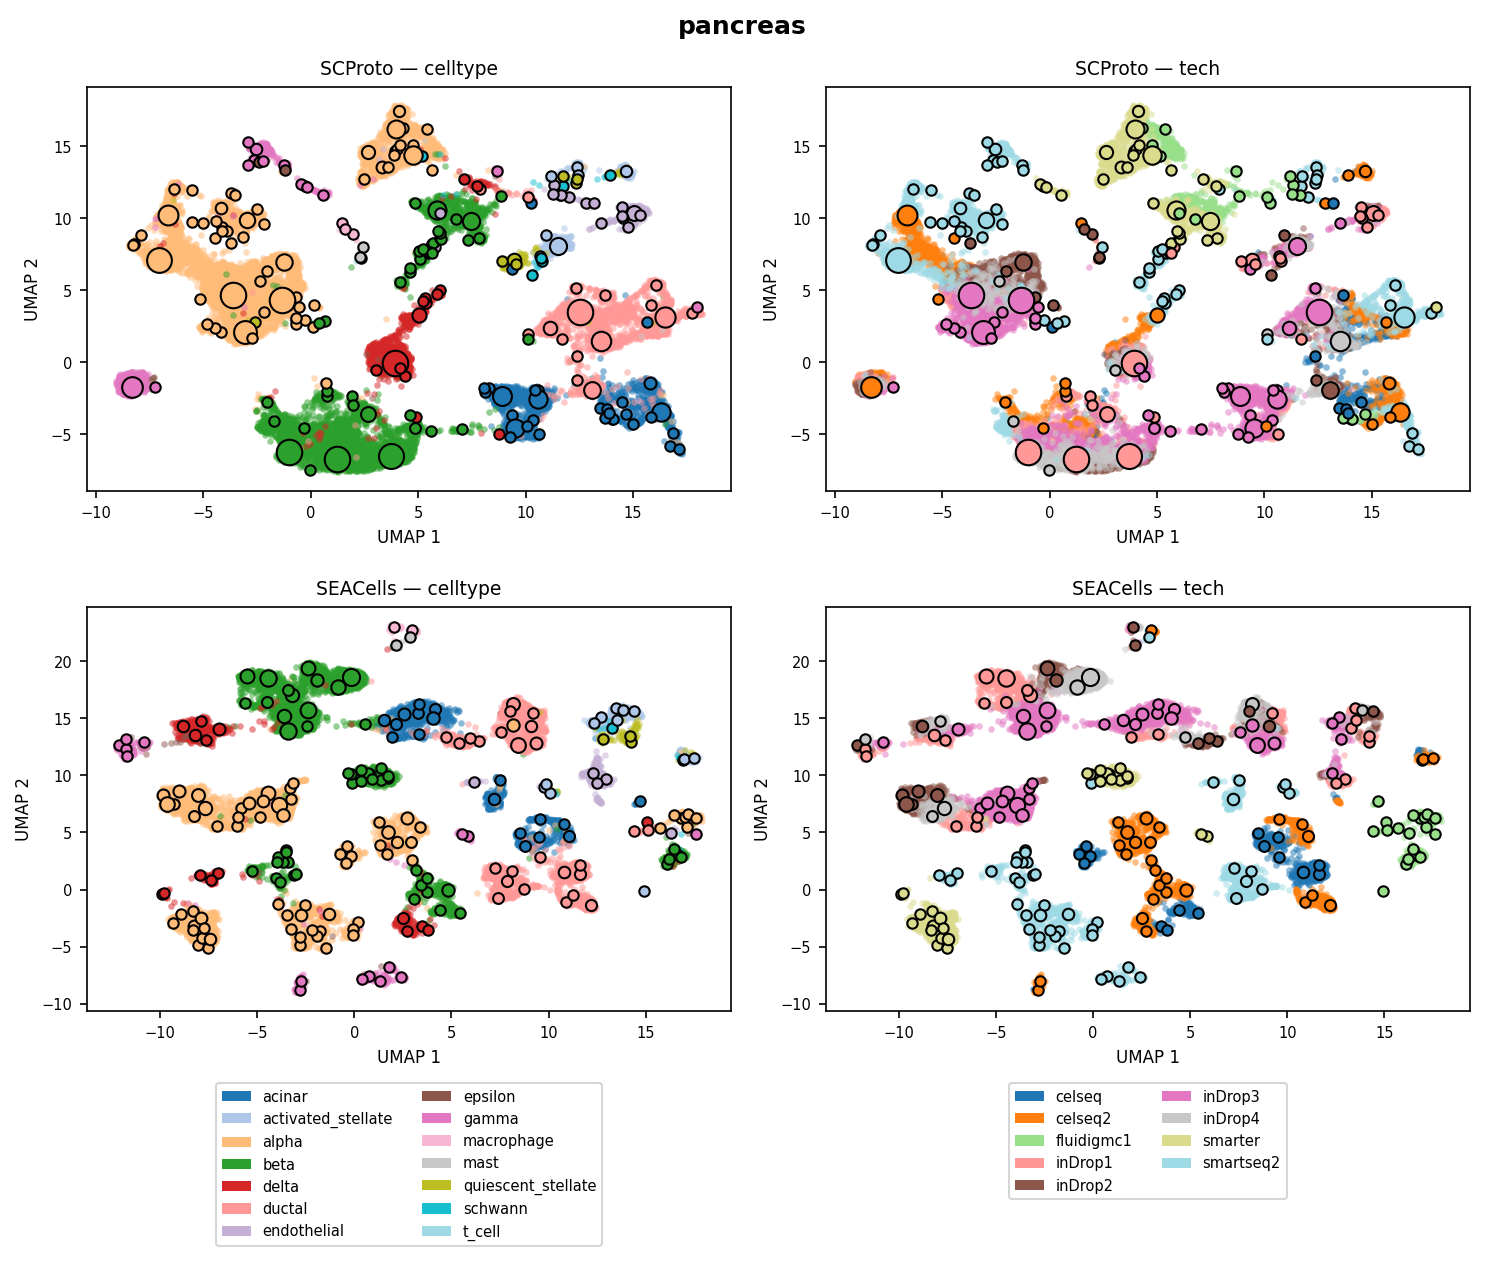
\includegraphics[width=\textwidth]{figures/pancreas_umap.png}
\caption{
UMAP visualization of metacells on the Pancreas dataset.
Top: SCProto. Bottom: SEACells.
Left: colored by cell type. Right: colored by batch (technology).
SCProto forms compact, biologically coherent clusters while mixing cells across batches.
SEACells produces batch-specific, fragmented metacells.
Black circles denote metacells (size proportional to number of assigned cells).
}
\label{fig:pancreas_umap}
\end{figure*}

\begin{table*}[t]
\centering
\caption{Graph preservation and cross-batch integration performance.
We report modularity (higher is better), batch entropy (higher indicates better mixing),
and cell-type purity (higher is better). Best results are in bold and second-best results are underlined.}
\label{tab:graph_batch}
\resizebox{\textwidth}{!}{%
\begin{tabular}{lccc|ccc|ccc}
\toprule
 & \multicolumn{3}{c}{Pancreas} 
 & \multicolumn{3}{c}{Immune} 
 & \multicolumn{3}{c}{Lung} \\
\cmidrule(lr){2-4} \cmidrule(lr){5-7} \cmidrule(lr){8-10}
Method 
& Modularity $\uparrow$ & Batch Entropy $\uparrow$ & Purity $\uparrow$
& Modularity $\uparrow$ & Batch Entropy $\uparrow$ & Purity $\uparrow$
& Modularity $\uparrow$ & Batch Entropy $\uparrow$ & Purity $\uparrow$ \\
\midrule

SCProto        
& $\underline{0.61 \pm 0.08}$ & $1.04 \pm 0.66$ & $\mathbf{0.98 \pm 0.07}$
& $\mathbf{0.62 \pm 0.08}$ & $\underline{0.94 \pm 0.51}$ & $0.87 \pm 0.13$
& $\underline{0.67 \pm 0.03}$ & $\mathbf{1.39 \pm 0.55}$ & $0.86 \pm 0.18$ \\

SEACells       
& $\mathbf{0.67 \pm 0.05}$ & $0.19 \pm 0.30$ & $\underline{0.97 \pm 0.08}$
& $\underline{0.55 \pm 0.04}$ & $0.16 \pm 0.24$ & $\mathbf{0.88 \pm 0.14}$
& $\mathbf{0.67 \pm 0.04}$ & $0.41 \pm 0.47$ & $\mathbf{0.90 \pm 0.15}$ \\

CVAE           
& $0.23 \pm 0.07$ & $\underline{1.38 \pm 0.41}$ & $0.97 \pm 0.07$
& $0.26 \pm 0.14$ & $0.81 \pm 0.40$ & $0.87 \pm 0.14$
& $0.32 \pm 0.05$ & $\underline{1.33 \pm 0.43}$ & $0.86 \pm 0.18$ \\

UMAP 
& $0.26 \pm 0.06$ & $\mathbf{1.51 \pm 0.37}$ & $0.94 \pm 0.10$
& $0.26 \pm 0.14$ & $0.80 \pm 0.40$ & $0.87 \pm 0.15$
& $0.32 \pm 0.06$ & $1.32 \pm 0.44$ & $0.86 \pm 0.18$ \\

\bottomrule
\end{tabular}}
\end{table*}

\begin{figure*}[t]
\centering
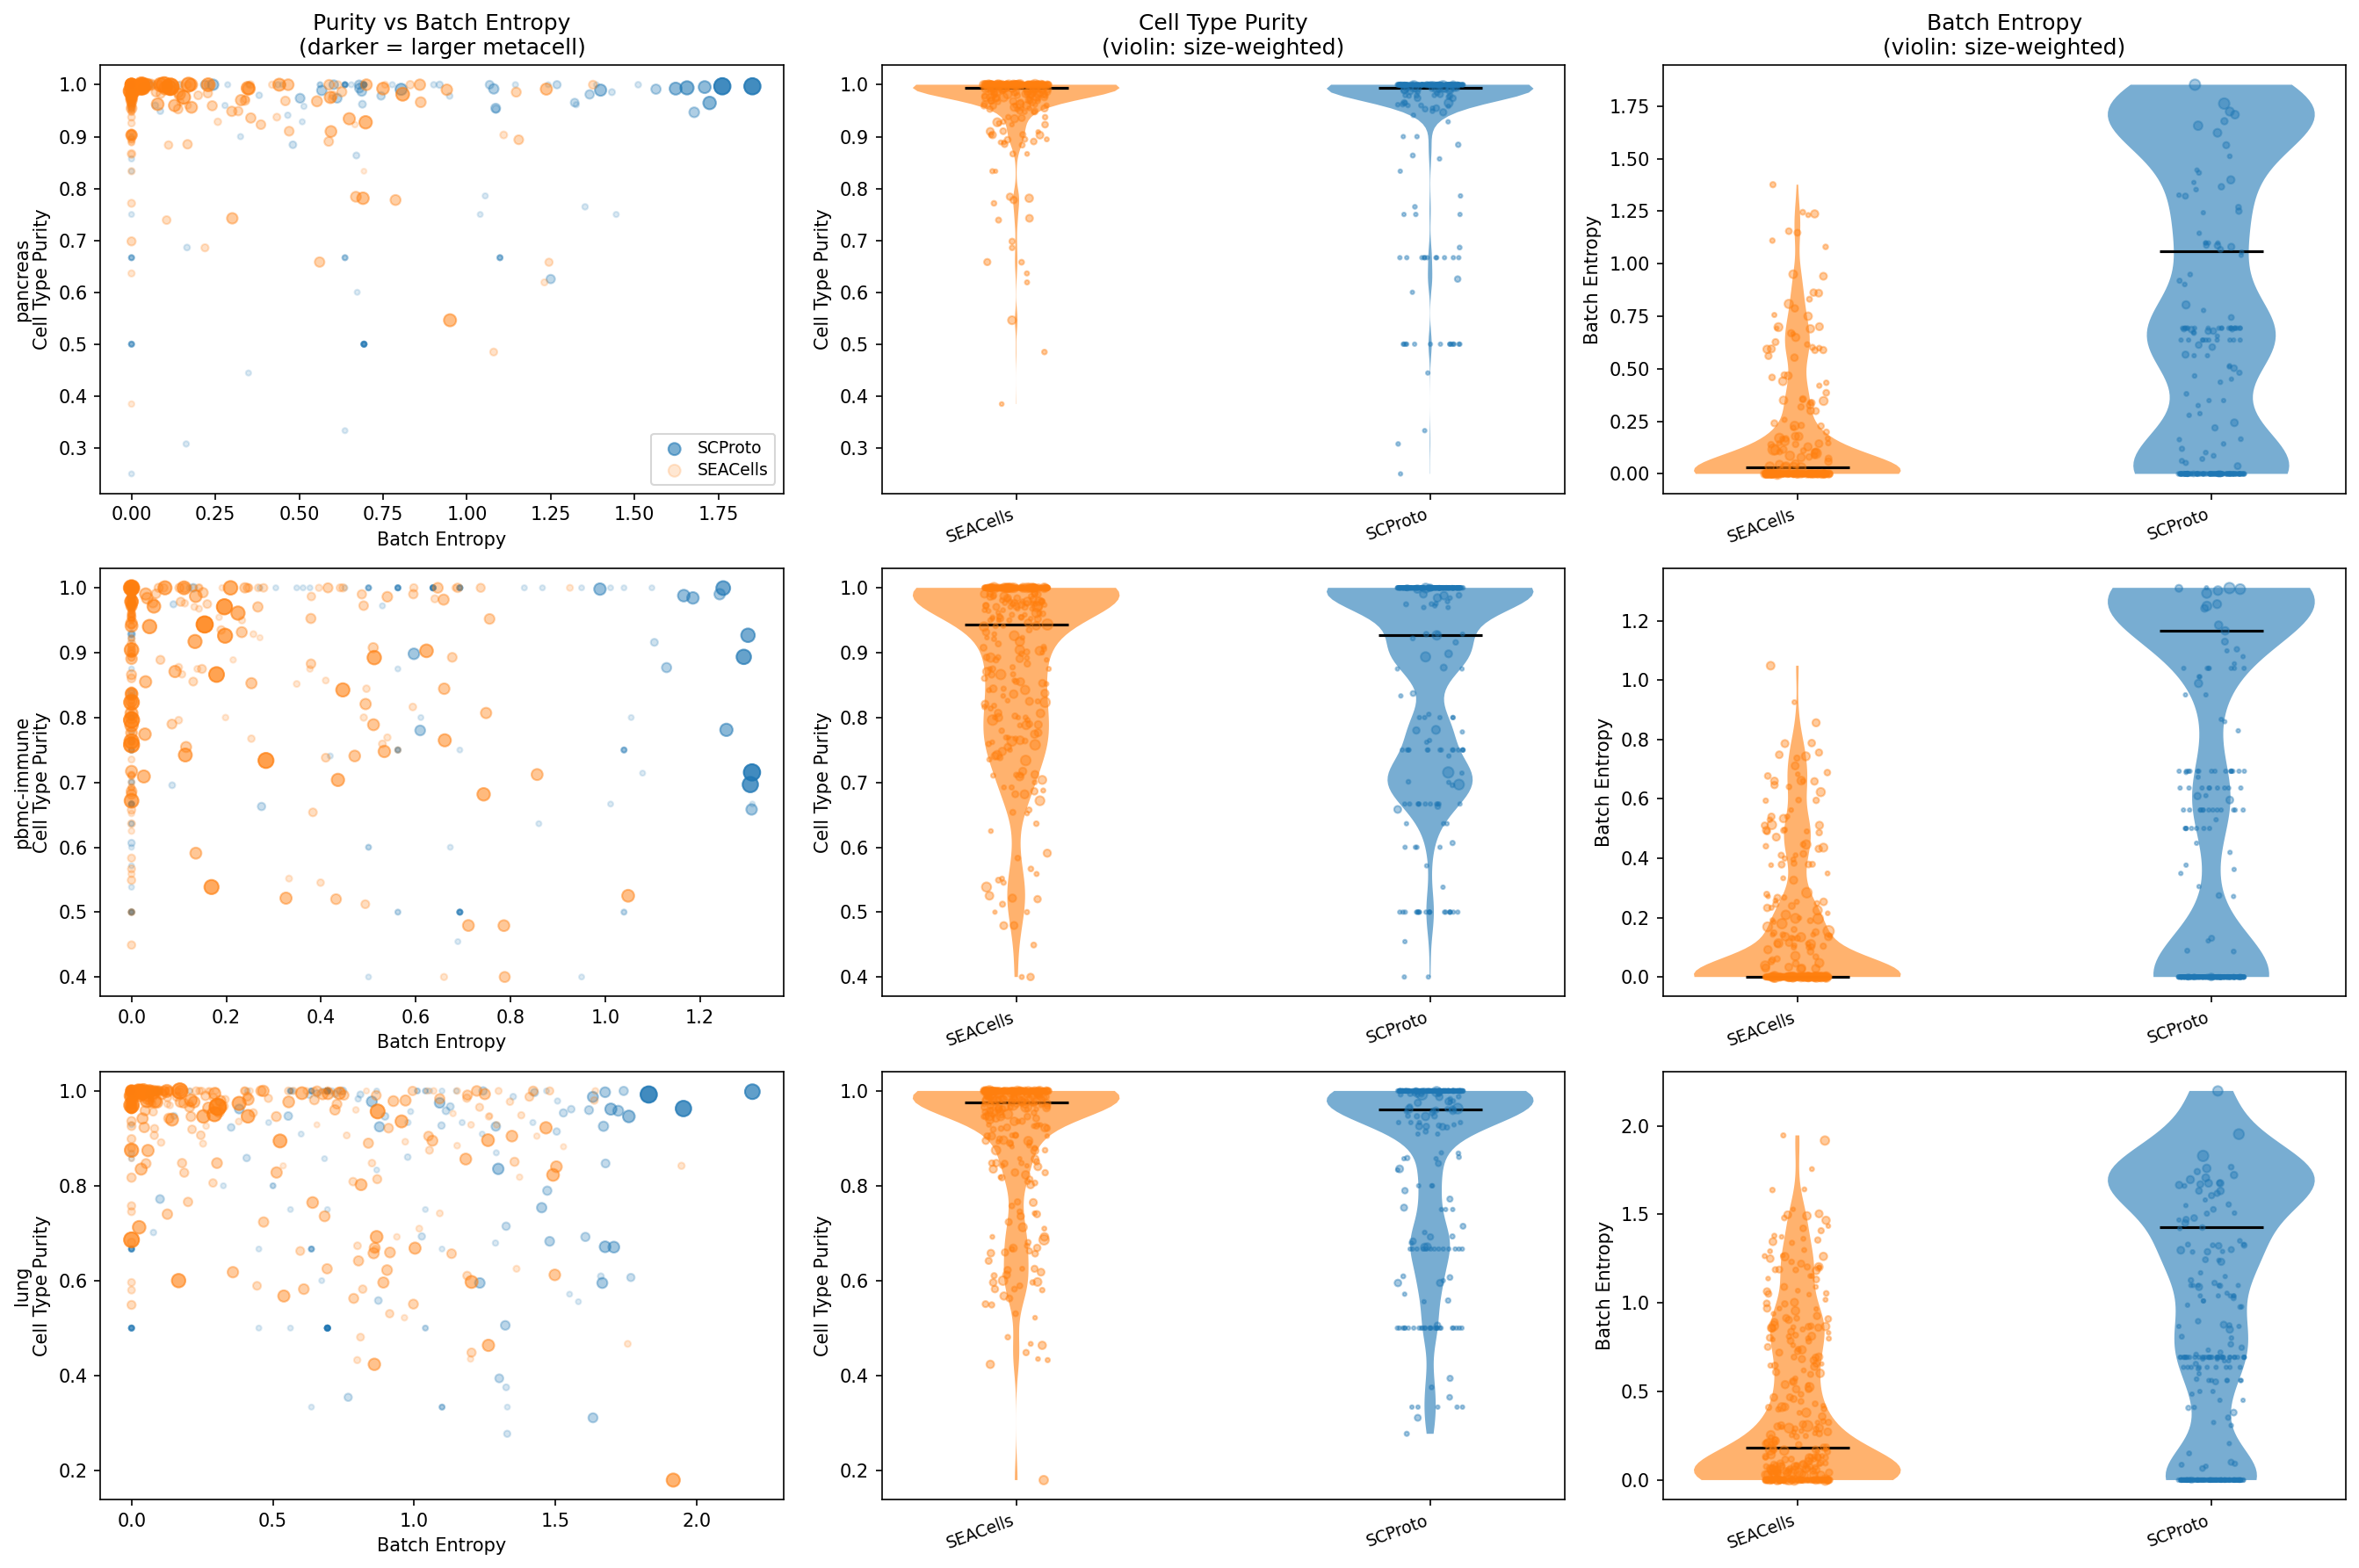
\includegraphics[width=\textwidth]{figures/pancreas_fig1.png}
\caption{
Per-metacell analysis of purity and batch mixing on the Pancreas dataset.
Left: Cell-type purity vs. batch entropy (point size proportional to metacell size).
Middle: Distribution of cell-type purity (size-weighted violin).
Right: Distribution of batch entropy (size-weighted violin).
SCProto achieves higher batch entropy while maintaining comparable purity to SEACells.
}
\label{fig:purity_entropy}
\end{figure*}


\subsection{Cross-Batch Metacells Improve Representation of Rare Cell Types}

We next evaluate whether cross-batch aggregation improves the representation of low-frequency (rare) cell types. We define rare cell types based on their overall frequency in the dataset (see Methods) and assess performance using (i) cell-type coverage, (ii) purity of metacells assigned to rare cell types, and (iii) the distribution of purity across frequency bins.

As shown in Table~\ref{tab:rare_cells}, SCProto achieves consistently higher or comparable coverage across datasets, indicating that aggregating cells across batches enables the formation of metacells for cell types that are underrepresented within individual batches. Importantly, SCProto also attains higher purity for metacells corresponding to rare cell types, demonstrating that it groups cells more coherently despite limited per-batch samples.

To further analyze performance across the frequency spectrum, we stratify cell types by frequency and evaluate metacell purity within each bin (Fig.~\ref{fig:rare_purity}). SCProto maintains high purity even for the rarest cell types, whereas SEACells shows a noticeable degradation in low-frequency bins. This suggests that restricting aggregation within batches limits the ability to form reliable metacells when only few samples are available per batch.

In contrast, reconstruction-based methods such as CVAE, and structure-preserving methods such as parametric UMAP, do not explicitly enforce community-level structure during training. As a result, they tend to merge rare cell states into larger, denser clusters, leading to reduced purity for low-frequency populations.

Together, these results demonstrate that cross-batch aggregation is critical for recovering rare cell states, enabling SCProto to construct accurate and biologically meaningful metacells even in low-sample regimes.

\begin{figure*}[t]
\centering
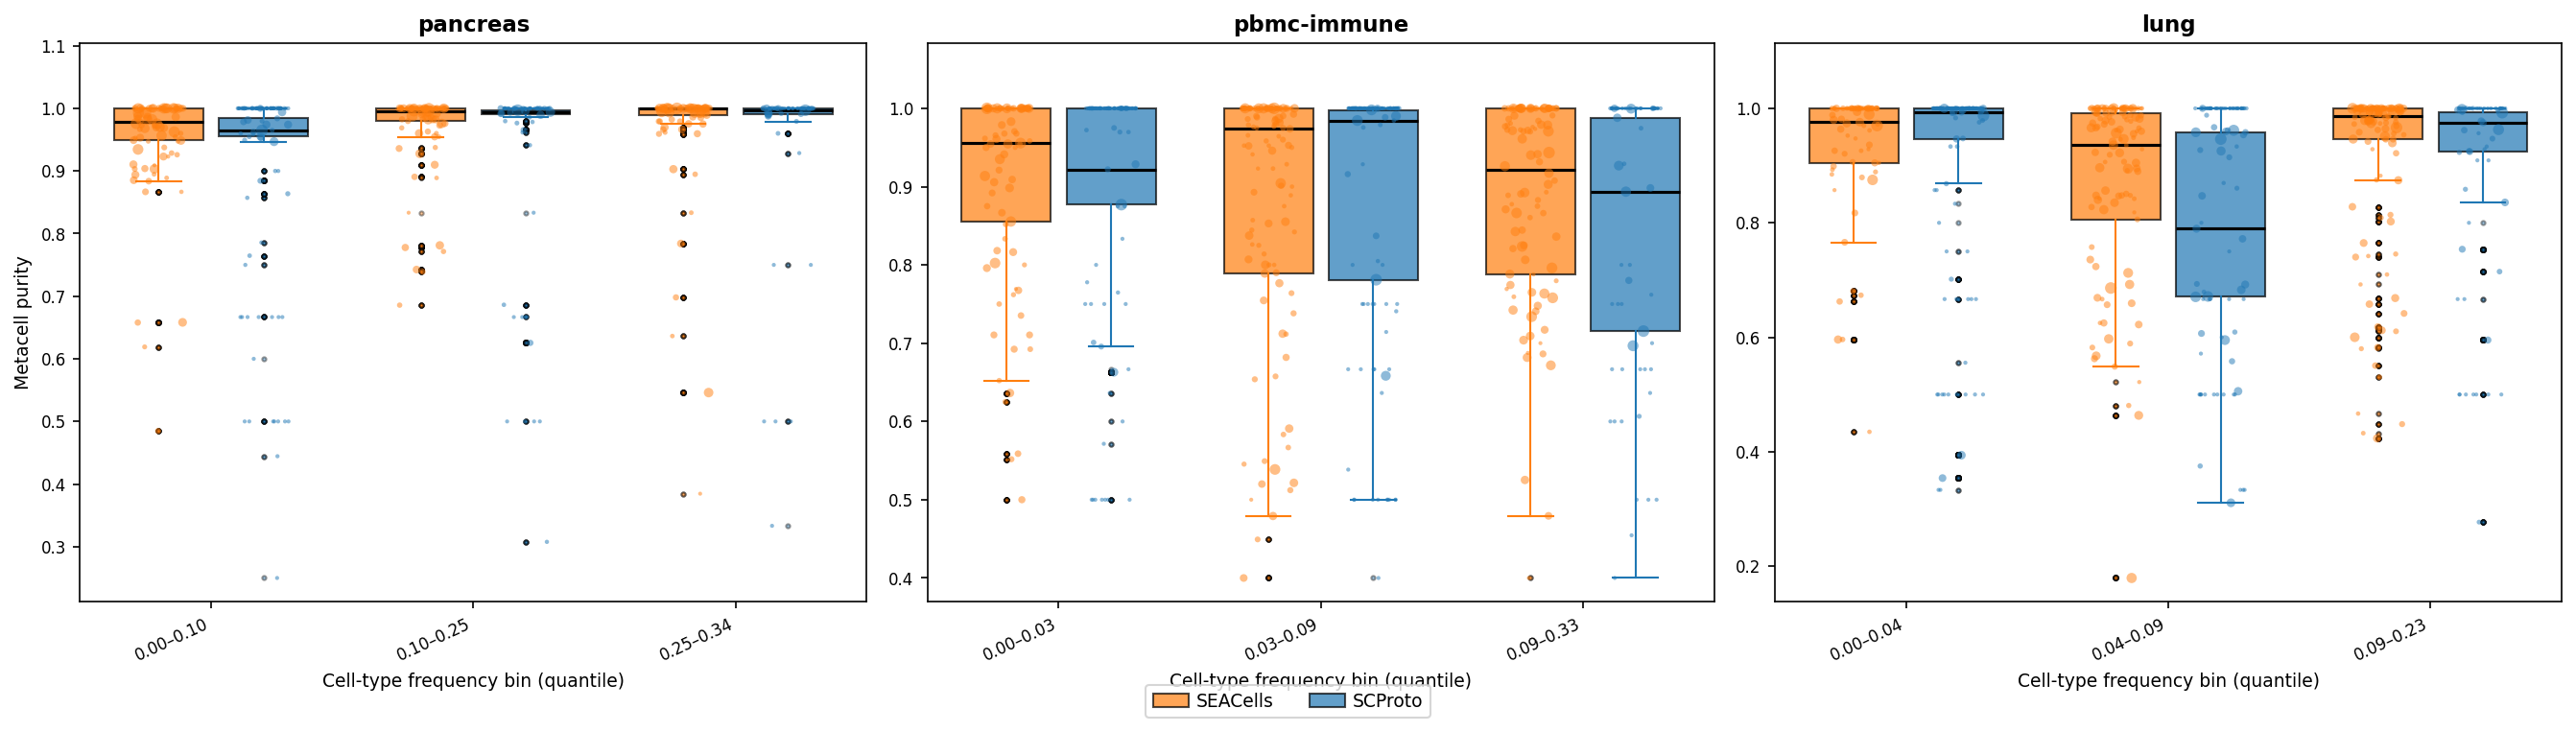
\includegraphics[width=\textwidth]{figures/freq_purities.png}
\caption{
Metacell purity stratified by cell-type frequency.
Cell types are grouped into frequency bins (quantiles), with lower-frequency bins corresponding to rare cell types.
Each point represents a metacell, and boxplots summarize the distribution.
SCProto maintains high purity across all frequency bins, while SEACells shows a clear degradation in purity for rare cell types.
}
\label{fig:rare_purity}
\end{figure*}

\begin{table*}[t]
\centering
\caption{Performance on rare cell types.
We report cell-type coverage (higher is better) and mean cell-type purity for low-frequency (rare) cell types (higher is better).}
\label{tab:rare_cells}
\resizebox{\textwidth}{!}{%
\begin{tabular}{lcc|cc|cc}
\toprule
 & \multicolumn{2}{c}{Pancreas} 
 & \multicolumn{2}{c}{Immune} 
 & \multicolumn{2}{c}{Lung} \\
\cmidrule(lr){2-3} \cmidrule(lr){4-5} \cmidrule(lr){6-7}
Method 
& Coverage $\uparrow$ 
& Rare Purity $\uparrow$ 
& Coverage $\uparrow$ 
& Rare Purity $\uparrow$ 
& Coverage $\uparrow$ 
& Rare Purity $\uparrow$ \\
\midrule

SCProto        
& 1.00 & $0.73 \pm 0.13$ 
& 1.00 & $0.88 \pm 0.13$ 
& 1.00 & $0.95 \pm 0.09$ \\

SEACells       
& 0.50 & $0.69 \pm 0.11$ 
& 1.00 & $0.90 \pm 0.10$ 
& 1.00 & $0.92 \pm 0.13$ \\

CVAE           
& 0.75 & $0.54 \pm 0.09$ 
& 0.75 & $0.58 \pm 0.21$ 
& 0.67 & $0.82 \pm 0.13$ \\

Parametric UMAP 
& 0.50 & $0.55 \pm 0.15$ 
& 1.00 & $0.61 \pm 0.12$ 
& 1.00 & $0.84 \pm 0.18$ \\

\bottomrule
\end{tabular}}
\end{table*}

\subsection{SCProto captures microenvironmental and spatial structure}

We evaluate whether incorporating spatial information enables SCProto to capture microenvironmental structure while preserving cell-type identity. To this end, we construct a spatial affinity graph based on local cellular neighborhoods and train SCProto using this graph. We compare against (i) SEACells trained on transcriptomic similarity, (ii) SEACells trained on the same spatial affinity graph, and (iii) a transcriptomics-only version of SCProto. Performance is assessed using both cell-type purity and niche purity.

As shown in Fig.~\ref{fig:spatial_heatmap}, SCProto achieves a strong balance between cell-type purity and niche purity, indicating that it captures spatially relevant structure without compromising biological identity. In contrast, SEACells trained on transcriptomic similarity fails to capture spatial organization, resulting in low niche purity. While SEACells trained on spatial affinity improves niche purity, it does so at the expense of cell-type purity, suggesting a loss of biological specificity.
\begin{figure*}[t]
\centering
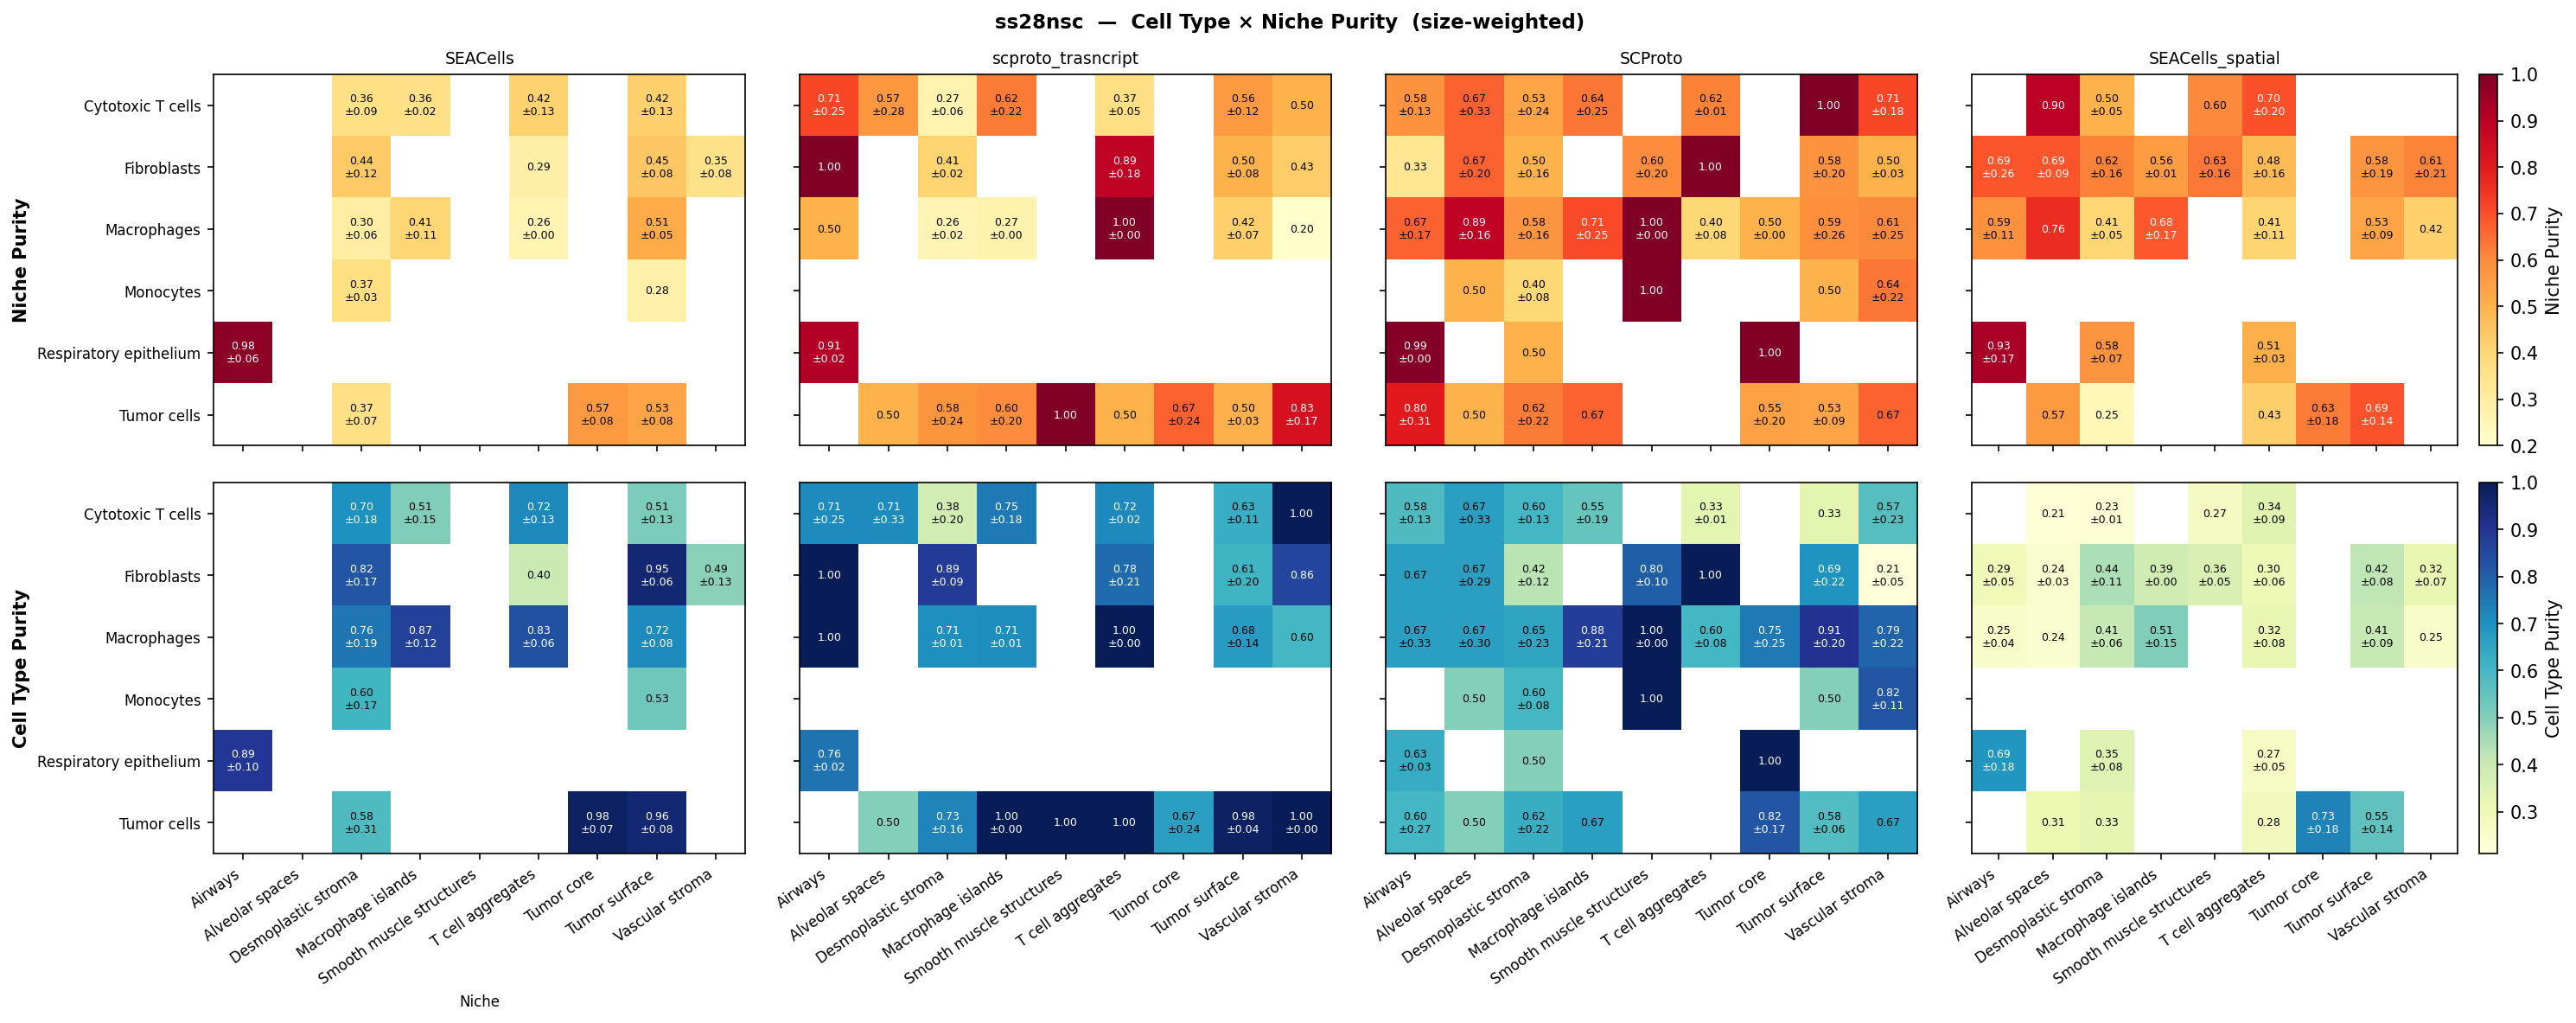
\includegraphics[width=\textwidth]{figures/heatmap.png}
\caption{
Cell type-- and niche-specific evaluation of niche purity and cell-type purity using size-weighted metrics.
Each entry shows mean $\pm$ standard deviation across metacells.
}
\label{fig:spatial_heatmap}
\end{figure*}


These differences are further illustrated in Fig.~\ref{fig:spatial}, where spatial visualizations show that SCProto groups cells from the same niches while maintaining coherent cell-type structure. This indicates that incorporating spatial affinity enables SCProto to capture gene expression patterns associated with microenvironmental context—signals that are not recoverable from transcriptomic similarity alone.
\begin{figure*}[t]
\centering
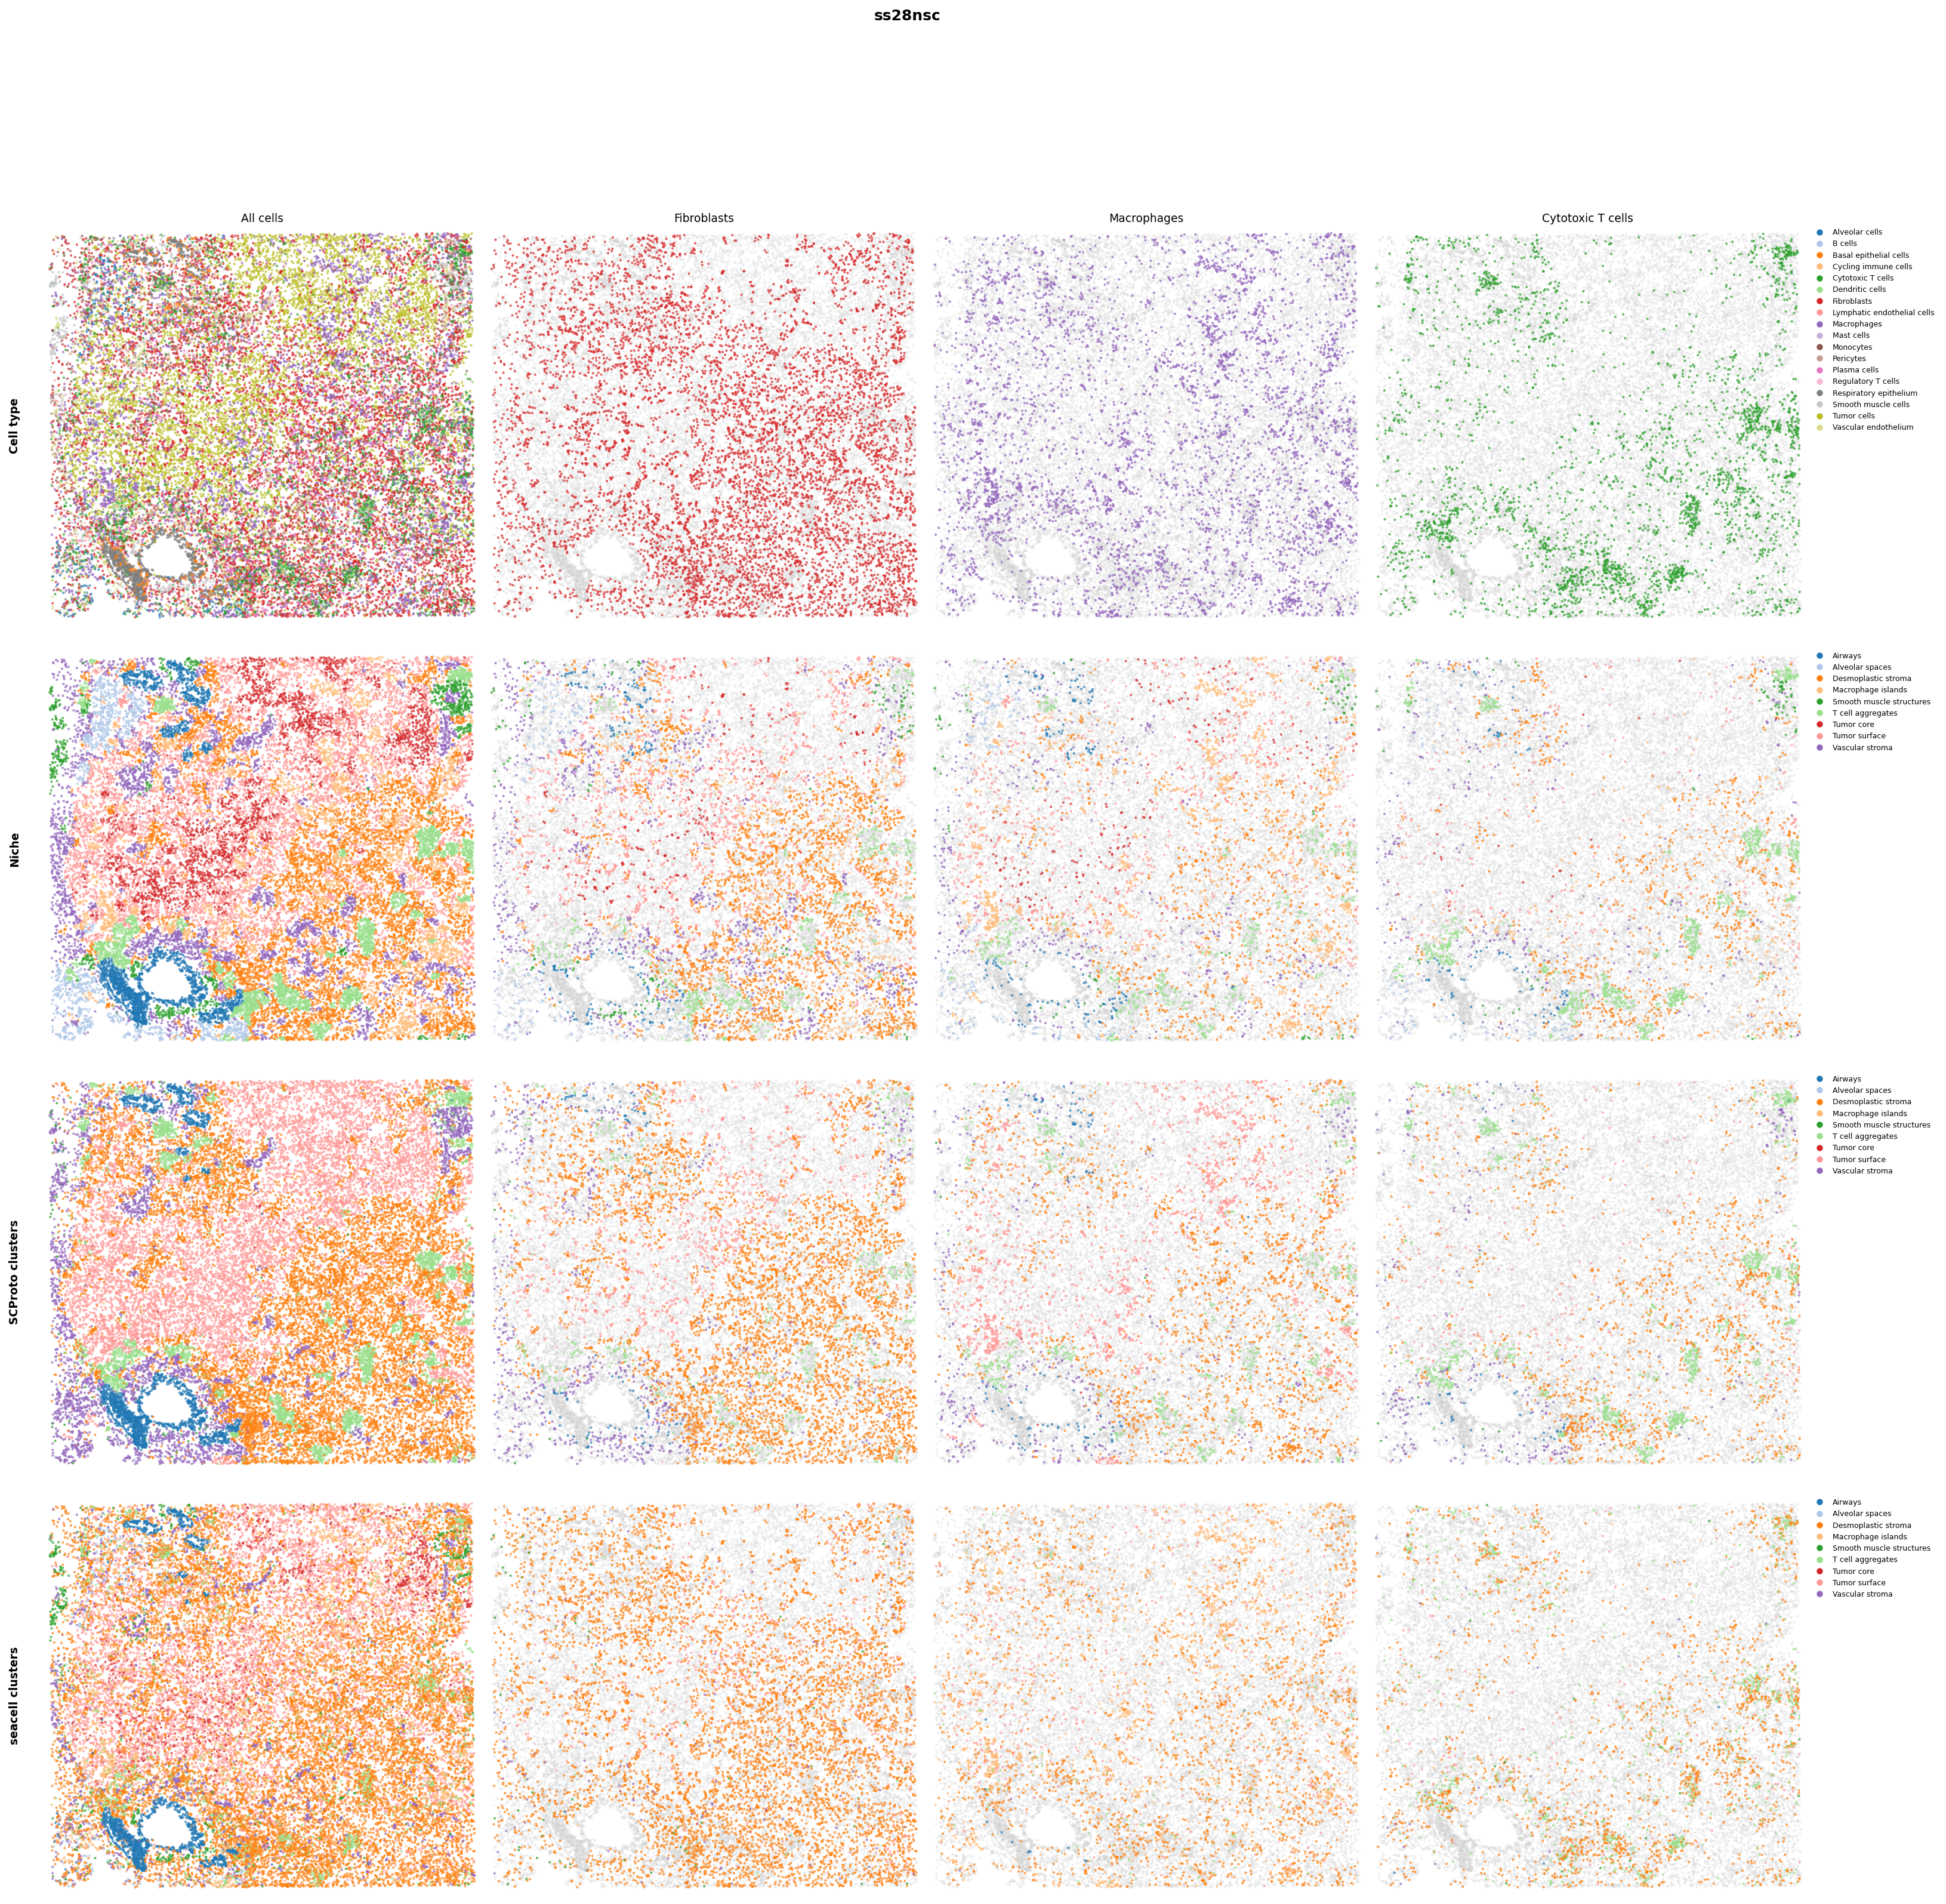
\includegraphics[width=\textwidth]{figures/spatial.png}
\caption{
Spatial visualization of cell types, niches, and metacell assignments across methods.
Columns correspond to selected cell types (fibroblasts, macrophages, cytotoxic T cells), and rows show cell-type annotations, niche annotations, SCProto metacells (trained on spatial affinity), and SEACells metacells (trained on the same affinity).
Each cell is colored by its assigned metacell.
SCProto produces spatially coherent patterns aligned with niche structure, while SEACells exhibits more fragmented patterns.
}
\label{fig:spatial}
\end{figure*}


Together, these results demonstrate that SCProto can flexibly integrate spatial information to learn metacells that reflect both cell identity and microenvironmental organization.

% \begin{figure*}[t]
% \centering
% 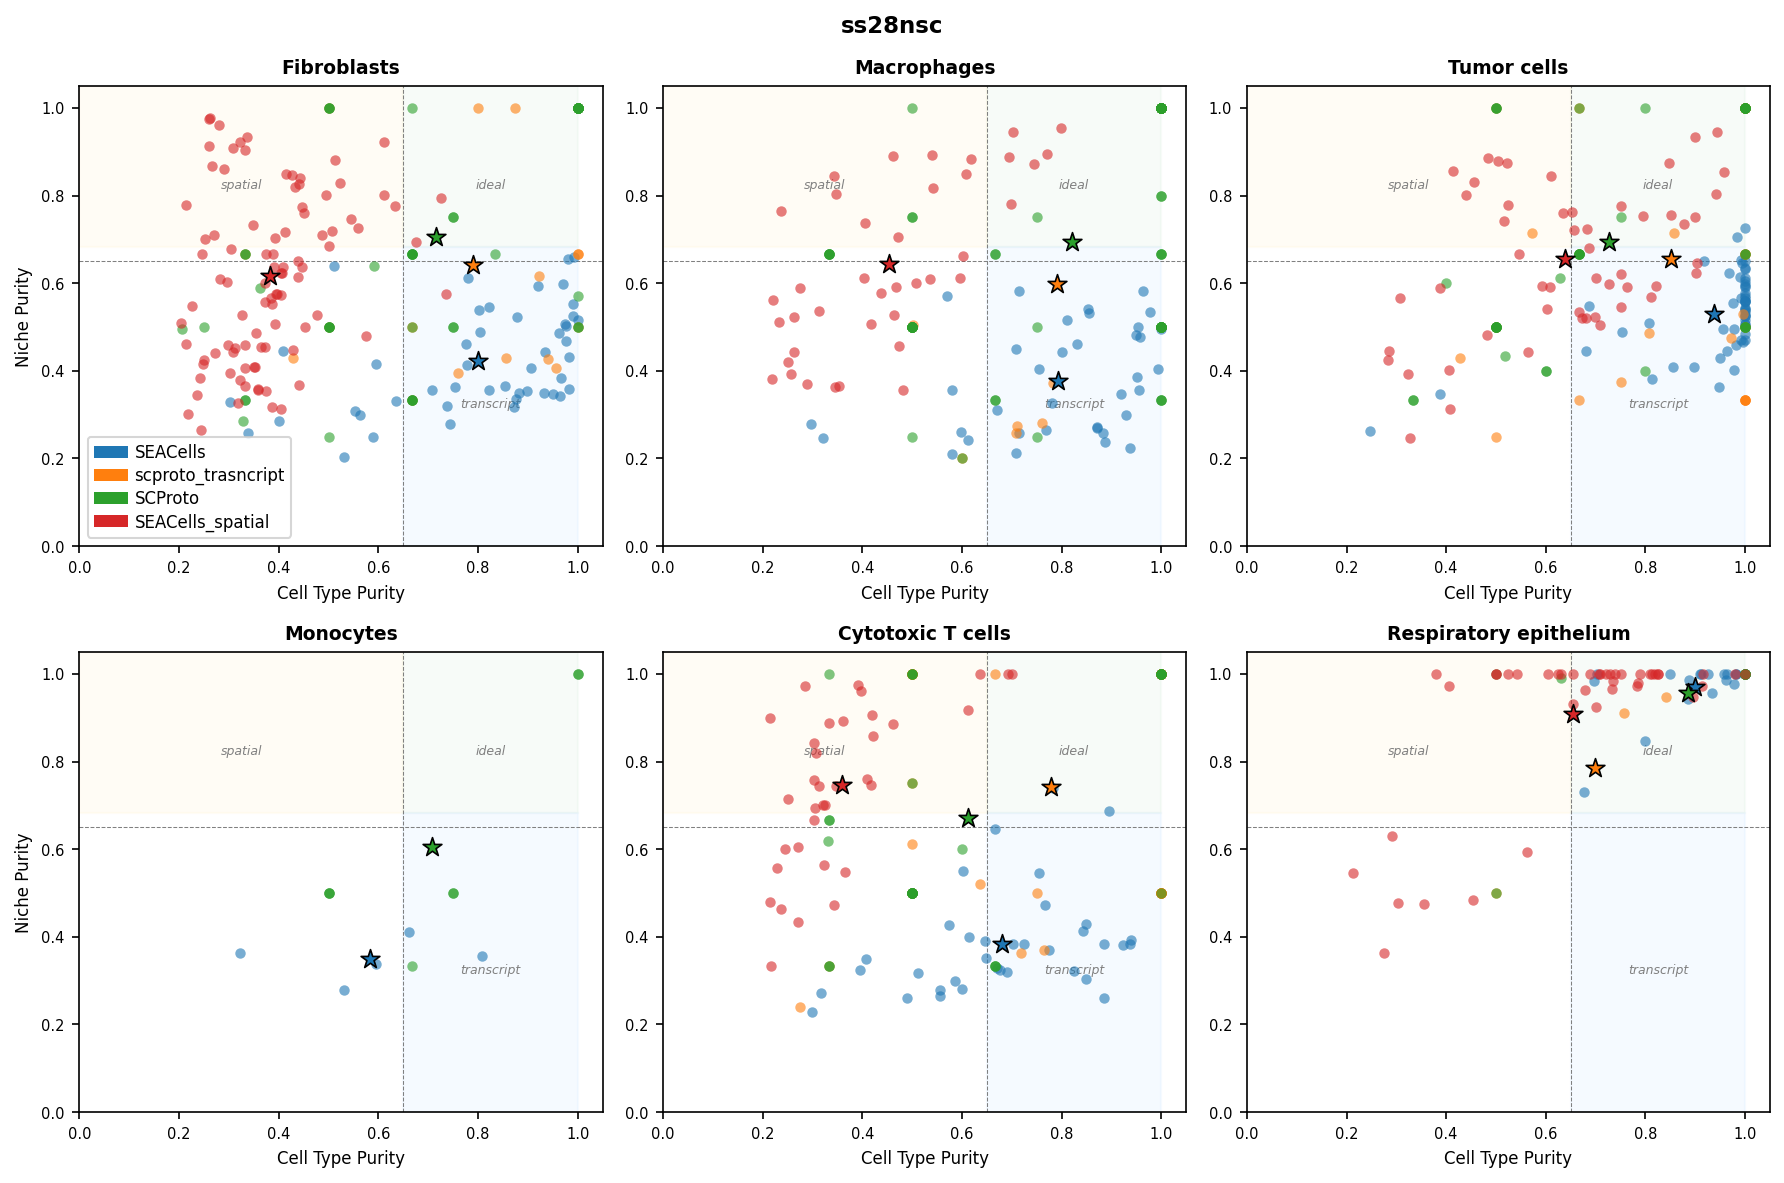
\includegraphics[width=\textwidth]{figures/tradeoff.png}
% \caption{
% Trade-off between cell-type purity and niche purity across metacells.
% Each point represents a metacell, colored by method, and star markers indicate method centroids.
% Arrows indicate the effect of incorporating spatial context by comparing SCProto trained on transcriptomic similarity with SCProto trained on spatial similarity.
% }
% \label{fig:spatial_tradeoff}
% \end{figure*}

% \begin{figure*}[t]
% \centering
% 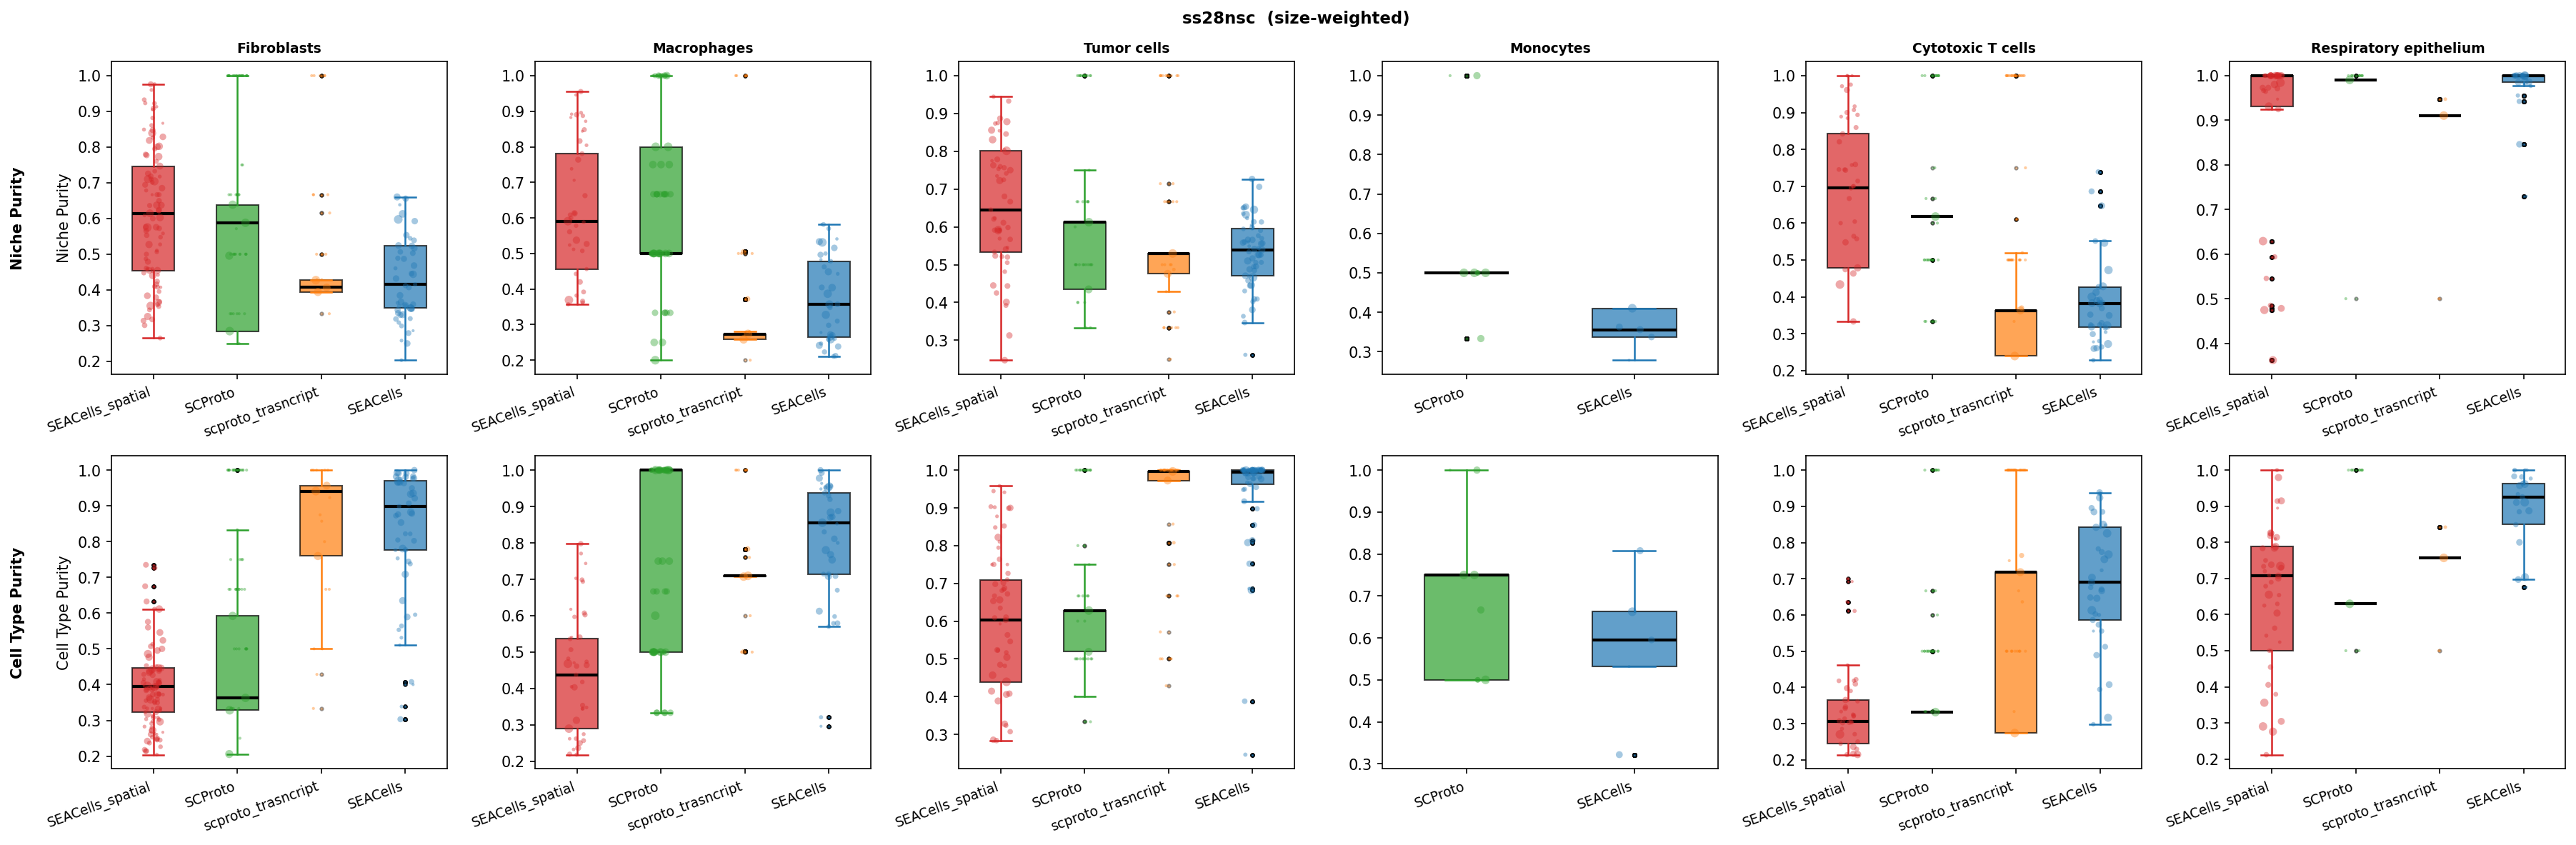
\includegraphics[width=\textwidth]{figures/niche_box.png}
% \caption{
% Comparison of niche purity and cell-type purity across methods for selected cell types using size-weighted metrics.
% SCProto improves niche purity compared to transcriptomics-only methods while maintaining substantially higher cell-type purity than the spatial SEACells baseline.
% }
% \label{fig:spatial_boxplots}
% \end{figure*}


